\documentclass[tikz,border=5pt]{standalone}
\usepackage{amsmath}
\usepackage{pgfplots}
\pgfplotsset{compat=1.18}
\usetikzlibrary{arrows.meta,calc}
\definecolor{ink}{HTML}{16324F}
\definecolor{teal}{HTML}{168A88}
\definecolor{gold}{HTML}{D9892B}
\definecolor{redq}{HTML}{B84A4A}
\begin{document}
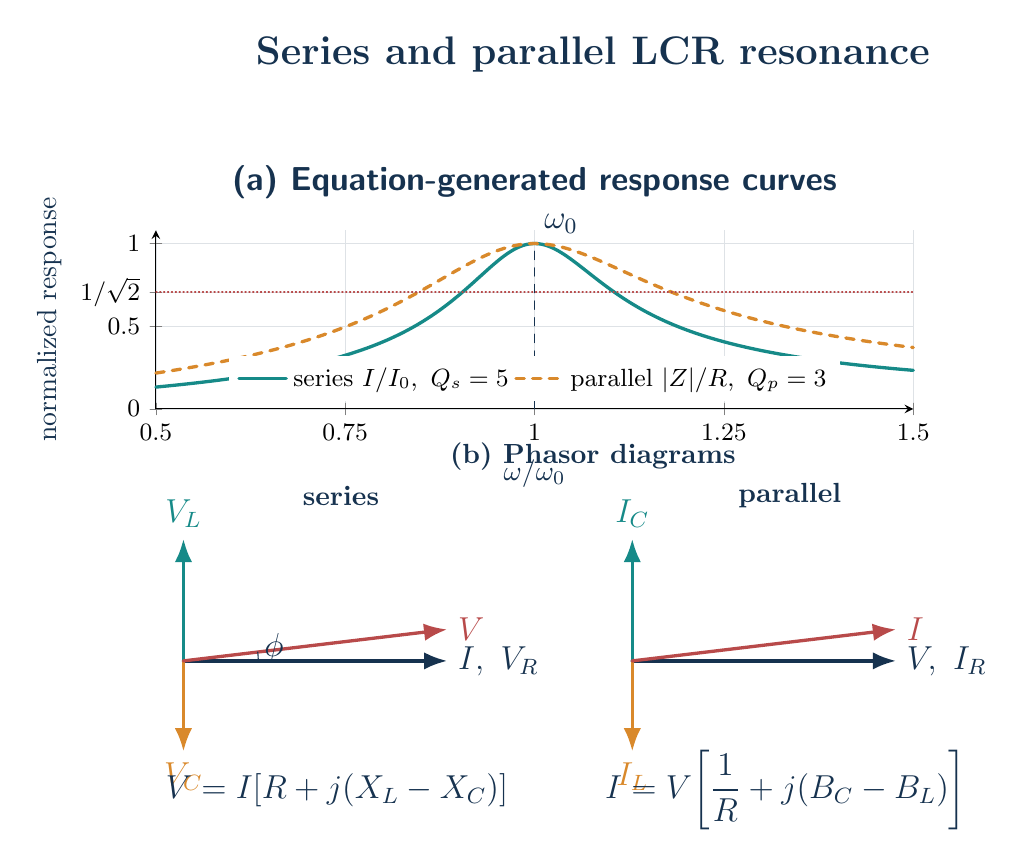
\begin{tikzpicture}[font=\large\sffamily,>=Latex,line cap=round,line join=round]
  \node[font=\bfseries\Large,ink] at (6.1,9.75)
    {Series and parallel LCR resonance};

  \begin{axis}[
    at={(.55cm,5.25cm)},anchor=south west,
    width=11.2cm,height=3.85cm,
    xmin=.5,xmax=1.5,ymin=0,ymax=1.08,
    axis lines=left,
    xlabel={$\omega/\omega_0$},ylabel={normalized response},
    xtick={.5,.75,1,1.25,1.5},
    ytick={0,.5,.7071,1},
    yticklabels={$0$,$0.5$,$1/\sqrt2$,$1$},
    grid=both,grid style={draw=ink!14,line width=.2pt},
    tick label style={font=\small},
    label style={font=\normalsize,ink},
    title={\bfseries (a) Equation-generated response curves},
    title style={ink,yshift=2pt},
    legend style={draw=none,fill=white,font=\small,at={(.5,.04)},anchor=south,legend columns=2},
    clip=false
  ]
    \addplot[teal,very thick,domain=.5:1.5,samples=360]
      {1/sqrt(1+25*(x-1/x)^2)};
    \addlegendentry{series \(I/I_0,\ Q_s=5\)}
    \addplot[gold,very thick,dashed,domain=.5:1.5,samples=360]
      {1/sqrt(1+9*(x-1/x)^2)};
    \addlegendentry{parallel \(|Z|/R,\ Q_p=3\)}
    \addplot[redq,densely dotted,domain=.5:1.5] {.70710678};
    \draw[ink,dashed] (axis cs:1,0)--(axis cs:1,1);
    \node[ink,above right] at (axis cs:1,1) {\(\omega_0\)};
  \end{axis}

  \node[font=\bfseries,ink] at (6.1,4.65) {(b) Phasor diagrams};
  \begin{scope}[shift={(.65,.25)}]
    \node[font=\bfseries,ink] at (2.25,3.9) {series};
    \coordinate (Os) at (.25,1.8);
    \draw[->,ink,very thick] (Os)--++(3.35,0) node[right] {$I,\ V_R$};
    \draw[->,teal,very thick] (Os)--++(0,1.55) node[above] {$V_L$};
    \draw[->,gold,very thick] (Os)--++(0,-1.15) node[below] {$V_C$};
    \draw[->,redq,very thick] (Os)--++(3.35,.40) node[right] {$V$};
    \draw[ink,thin] ($(Os)+(.95,0)$) arc[start angle=0,end angle=6.8,radius=.95];
    \node[ink] at ($(Os)+(1.15,.16)$) {$\phi$};
    \node[ink,align=center] at (2.2,.16)
      {$\displaystyle V=I\!\left[R+j(X_L-X_C)\right]$};
  \end{scope}

  \begin{scope}[shift={(6.35,.25)}]
    \node[font=\bfseries,ink] at (2.25,3.9) {parallel};
    \coordinate (Op) at (.25,1.8);
    \draw[->,ink,very thick] (Op)--++(3.35,0) node[right] {$V,\ I_R$};
    \draw[->,teal,very thick] (Op)--++(0,1.55) node[above] {$I_C$};
    \draw[->,gold,very thick] (Op)--++(0,-1.15) node[below] {$I_L$};
    \draw[->,redq,very thick] (Op)--++(3.35,.40) node[right] {$I$};
    \node[ink,align=center] at (2.2,.16)
      {$\displaystyle I=V\!\left[\frac1R+j(B_C-B_L)\right]$};
  \end{scope}
\end{tikzpicture}
\end{document}
